\documentclass[m]{vakthesis}

\usepackage[T2A]{fontenc}
\usepackage[utf8]{inputenc}
\usepackage[english,russian,ukrainian]{babel}

%\usepackage{graphicx}
\usepackage{subfigure}
\usepackage{alltt}
\usepackage{moreverb}
\usepackage{setspace}
\usepackage{algorithmic}
\usepackage{algorithm}
\usepackage{multirow}
\usepackage{bigstrut}
\usepackage{makecell}
\usepackage[table]{xcolor}
\usepackage{tabularx}
\usepackage[pdftex]{graphicx}


\usepackage{url}
\usepackage{array}
\usepackage{booktabs}

\usepackage[intlimits]{amsmath}
\allowdisplaybreaks
\usepackage{amsthm}
\usepackage{amssymb}

\usepackage{geometry}
\geometry{hmargin={30mm,15mm},vmargin={26mm,26mm}}

\usepackage[version=0.96]{pgf}
\usepackage{tikz}
\usetikzlibrary{arrows,shapes,shapes.arrows,shapes.misc,snakes,automata,backgrounds,petri,patterns,positioning,scopes,chains,matrix,decorations.pathmorphing,shadows}

\def\argmin{\mathop{\rm arg\,min}}

\theoremstyle{plain}
\newtheorem{theorem}{Теорема}[chapter]
\newtheorem{lemma}{Лема}[chapter]
\newtheorem{corollary}{Наслідок}[chapter]
\theoremstyle{definition}
\newtheorem{definition}{Означення}[chapter]
\newtheorem{example}{Приклад}[chapter]
\theoremstyle{remark}
\newtheorem{remark}{Зауваження}[chapter]
\theoremstyle{statement}
\newtheorem{statement}{Твердження}[chapter]

\begin{document}

\tikzset{
  terminal/.style={
    % The shape:
    rounded rectangle,
    minimum size=6mm,
    % The border:
    very thick,
    draw=green!50!black!50,         % 50% red and 50% black,
                                  % and that mixed with 50% white
    % The filling:
    top color=white,              % a shading that is white at the top...
    bottom color=green!50!black!20, % and something else at the bottom
    % Font
    font=\itshape,text centered
  },
  process/.style={
    % The shape:
    rectangle,
    % The size:
    minimum size=6mm,
    % The rest
    very thick,draw=black!50,
    top color=white,bottom color=black!20,
    font=\ttfamily,text centered
  },
  decision/.style={
    % The shape:
    diamond, 
    minimum size=6mm,    
    % The rest
    very thick,draw=black!50,
    top color=white,bottom color=black!20,
    font=\ttfamily,text centered
  },
  data/.style={
    % The shape:
    trapezium,
    trapezium left angle=70, 
    trapezium right angle=110,    
    minimum size=6mm,    
    % The rest
    very thick,draw=black!50,
    top color=white,bottom color=black!20,
    font=\ttfamily,text centered
  },
  line/.style={draw, very thick, color=black!50,rounded corners},
  help-lines/.style={draw, very thin, color=black!50},
  arrow/.style={draw, very thick, color=black!50, -latex',rounded corners},
  helper-arrow/.style={draw, very thin, color=black, -latex'},
  dashed-line/.style={draw, dashed, color=black},
  point/.style={coordinate}
}
\floatname{algorithm}{Алгоритм} 
\title{Методи кластеризації на великих масивах даних}
\author{Волощук Орест Романович}
\supervisor{Притула Микола Миколайович}
           {проффесор}
\supervisor{Годич Олесь Васильович}
           {кандидат фізико-математичних наук, доцент}
       
\speciality{01.05.03}
\udc{004.853+004.855.5}
\institution{Львівський національний університет імені~Івана~Франка,Міністерство освіти та науки молоді і спорту України}{Львів}
\date{2011}


\maketitle

\setcounter{tocdepth}{2}
\tableofcontents
\nocite{*}

\graphicspath{{./images/}}

\chapter*{Вступ}

\paragraph{Актуальність теми}

Сьогодні все частіше виникають задачі, так чи інакше пов'язані із розбиттям масиву об'єктів на групи за певними критеріями. Із розвитком обчислювальної техніки збільшуються також об'єми баз даних, що можуть піддаватись такому аналізу. Виникає необхідність створення ефективних алгоритмів опрацювання великих масивів даних.

\paragraph{Мета і завдання дослідження}

Метою дослідження є оптимізація алгоритмів кластеризації для обробки великих масивів даних.
Для досягнення цієї мети були сформульовані та вирішені такі основні завдання:
\begin{itemize}
    \item провести порівняльний аналіз алгоритмів кластеризації
    \item розробити методи та виявити покращення, що дозволять прискорити виконання задачі кластеризації
    \item здійснити оцінку покращення роботи алгоритмів кластеризації за рахунок здійсненої оптимізації
\end{itemize}

\subparagraph{Об'єкт дослідження}
Об’єктом дослідження є процеси ієрархічної та роздільної кластеризації даних великих об’ємів.

\subparagraph{Предмет дослідження}
Предметом дослідження є оптимізація алгоритмів кластеризації для ефективного аналізу даних великих об’ємів.

\chapter{Огляд стану проблеми та основні поняття}\label{ch:01}

\section{Історія кластеризації}
    Термін ,,кластерний аналіз'', вперше використаний Тріоном у \cite{Tryon:Cluster:1939}, означає набір підходів та алгоритмів, призначених для об'єднання схожих об'єктів у групи. Ця технологія знайшла своє застосування в цілій низці галузей наук та є необхідною частиною більшості сучасних засобів аналізу даних.
 
    В 1959 радянський вчений Терентьєв розробив так званий ,,метод кореляційних плеяд'' \cite{Terentyev}, покликаний здійснювати групування на базі корелюючих ознак об'єктів. Займаючись вивченням кореляцій між різними ознаками озерної жаби, він об'єднав їх в групи за абсолютною величиною коефіцієнту кореляції. Таким чином він отримав дві групи ознак -- ознаки із великим та з малим значенням кореляції. Терентьєв назвав ці групи ,,кореляційними плеядами'' та опублікував декілька методів їх аналізу. Це посприяло розвитку методів кластеризації за допомогою графів.
    
    На початку 50х років також вийшли публікації Р.~Льюїса, Е.~Фікса та Дж.~Ходжеса, присвячені ієрархічним алгоритмам кластеризації. Відчутний поштовх технології кластерного аналізу дали роботи Розенблатта про розпізнаючий пристій ,,перцептрон'', котрі поклали початок теорії ,,розпізнавання без вчителя''. Поштовхом до розробки методів кластеризації стала публікація \cite{SokalSneath} в 1963 році. В своїй роботі автори виходили з того, що для створення ефективних біологічних класифікацій процедура кластеризації повинна використовувати всеможливі показники, що характеризують досліджувані організми, проводити оцінку ступеня схожості між цими організмами, та забезпечувати розташування схожих організмів в одну групу. При цьому сформовані групи повинні бути досить локальними, тобто схожість організмів всередині групи повинна бути більшою, ніж між групами. Подальший аналіз таких груп допоможе вияснити, чи відповідають вони реальним біологічним класифікаціям. Сокел та Сніт, автори цеї роботи, вважали, що виявлення структури розподілу об'єктів у групи допоможе встановити процес утворення цих груп.
    
    В середині сімдесятих з'явилась також низка робіт, присвячених методам аналізу якості здійсненої кластеризації. Індекси Данна \cite{Dunn}, Девіса-Боулдіна \cite{DavisBouldin} певною мірою дозволяють оцінити придатність результатів таксономії до реального використання.
    
    в цей період розвитку технології ще не приділялось великої уваги необхідності передбачення можливості масштабування алгоритмів. Вибірки, що піддавались кластеризації, не були настільки великими, щоб масштабування мало зміст.

\section{Типові задачі}
    Із кластерів, що повертаються в результаті роботи алгоритмів таксономії, можна виділити типових представників , і надалі працювати не з кожним об'єктом великого масиву, а лише з цими представниками. Це дозволяє суттєво спростити аналіз даних. Кластеризація часто стає складовою якоїсь більшої задачі, інструментом підготовки даних для її розв'язання. Такі задачі завжди пов'язані із пошуком та виділенням змістовних структур із великих масивів даних. 

    До них можна віднести задачі сегментування та розпізнавання зображень, мовлення, пошуку прихованих закономірностей в даних. На практиці такі задачі виникають при розв'язуванні проблем, що виникають в медицині, соціології, економіці та низці інших сфер діяльності людини. 
     медицині, наприклад, техніка сегментування зображення дозволяє виділяти на томограмах окремі області і на підставі їх форми та забарвлення приймати ставити діагноз. 
    В біології використовуються техніки кластеризації для виявлення взаємопов'язаних груп генів та їх впливу на живі організми. 
    Кластеризація успішно застосовується у маркетингових дослідженнях для виявлення зв'язків між різними групами споживачів та потенційних покупців, цільових аудиторій, та оптимального позиціонування нової продукції. 
    В соціологічних дослідженнях використовується кластеризація даних, отриманих з різних джерел, для спрощення їх подальшого аналізу. 

    У своїй праці \cite{Zagorujko} Загоруйко описує одну із таких задач. Новосибірські вчені вивчали причини переселення людей з сіл в міста. Були вислані експедиції в навколишні села, жителям яких задавали приблизно сто анкетних питань, що стосувались віку, сімейного становища, освіти та ін. Після завершення опитування дослідники постали перед необхідністю аналізувати більш ніж сім тисяч анкет, що містили понад сто питань кожна. 
    Ці дані було введено в програму таксономії, котра повернула сім великих таксонів, середні характеристики яких дозволили дати зібраним даним змістовну інтерпретацію. Наприклад, виділився кластер, що містив переважно жінок середнього віку, котрі мали дорослих дітей в місті. Очевидно, представниці цього таксону, названого дослідниками ,,бабусі'', їхали в місто доглядати за своїми внуками. Решту таксонів опрацьовано аналогічно.
    
    Перед процедурою кластеризації часто дані буває необхідно підготувати. В практиці нормою є випадки, коли для деяких об'єктів бракує частини атрибутів -- в такому разі перед кластеризацією необхідно здійснити передбачення цих атрибутів, користуючись наявною інформацією. Також значення атрибутів об'єктів необхідно нормувати.

\section{Основні поняття та означення}
    Дамо математичне означення кластеризації. Нехай $D$ -- множина об'єктів. 
    \begin{definition}
        \emph{Кластеризацією} $C = \{C \mid C \subseteq D\}$ називається таке розбиття $D$ на множини, 
        для якого виконується $\cup_{C_i \in C} = D$ і $\forall C_i, C_j \in C : C_i \cap C_{j \neq i} = \emptyset$. 
        Множини $C_i$ називаються кластерами.
    \end{definition}
    Як вже згадувалось раніше, задача кластеризації полягає в знаходженні такого розбиття $C$, щоб схожі між собою об'єкти належали до одного кластера, а не схожі - до різних. Необхідно визначити спосіб обчислення схожості об'єктів.
    Для цього на просторі об'єктів вводиться певна метрика, геометричний зміст якої -- відстань між об'єктами. Вона використовується як величина, обернена до міри схожості між об'єктами. На даний момент розроблено і широко застосовується наступний набір метрик:
    \begin{itemize}
        \item {евклідова відстань} 
            \[ 
                \rho(x, x') = \sqrt{ \sum_{i=1}^n (x_i - x_i')^2}
            \]
        \item {квадрат евклідової відстані} 
            \[
                \rho(x, x') = \sum_{i=1}^n (x_i - x_i')
            \]            
            (використовується для надання більшої ваги об'єктам, розташованим далеко один від одного)
        \item {манхеттенська відстань} 
            \[
                \rho(x, x') = \sum_{i=1}^n \mid x_i - x_i' \mid
            \]
        \item {відстань Чебишева}
            \[
                \rho(x, x') = max(\mid x_i - x_i' \mid )
            \]            
            ця метрика дозволяє розрізнити об'єкти, якщо вони відрізняються лише одною координатою
    \end{itemize}
    
    
    
\section{Алгоритми кластеризації}
    На даний момент значного розвитку набула ціла низка різноманітних алгоритмів кластеризації. Їх можна розділити на групи за різними ознаками:
    \begin{itemize}
        \item спосіб групування
            \begin{itemize}
                \item плоскі
                \item ієрархічні
            \end{itemize}
        \item визначеність 
            \begin{itemize}
                \item визначені
                \item невизначені
            \end{itemize}
        \item чутливість до форми кластерів 
            \begin{itemize}
                \item кластери мають строго сферичну форму
                \item кластери можуть мати довільну форму
            \end{itemize}
    \end{itemize}
    
    Плоскі алгоритми будують одне розбиття вибірки на кластери. На відміну від них, агломеративні будують цілу систему взаємовкладених кластерів. На виході алгоритму отримується дерево кластерів, коренем якого служить кластер, що містить усі об'єкти вибірки, а листками є найменші кластери з одним об'єктом кожен. В такому разі дослідник має можливість обрати такий переріз дерева, що найкраще відповідатиме його потребам.
    
    Визначені алгоритми однозначно ставлять у відповідність кожному об'єкту один кластер. Невизначені не дають такої чіткої інформації. Замість ідентифікатора кластера вони повертають імовірність, із якою об'єкт належить до кожного із кластерів.
    
    На сьогоднішній день широко використовуються наступні алгоритми кластеризації:
    \begin{itemize}
        \item k-means (\cite{Steinhaus}, \cite{MacQueen})
        \item UPGMA (\cite{SokalMichener})
        \item DBScan
        \item FOREL (\cite{Zagorujko})
        \item c-means
        \item карти Кохонена (\cite{Rosenblatt})
    \end{itemize}

\chapter {Аналіз алгоритмів}

    В даній роботі розглядається ефективність чотирьох алгоритмів кластеризації. Два із них здійснюють роздільну кластеризацію: k-means та DBSCAN. Інші два --- ієрархічну: UPGMA та споріднений із ним Neighbor-joining.

    \section {Опис алгоритмів}
        \paragraph {K-Means}
            K-means --- це метод кластеризації, що повертає таке розбиття, в якому кожен об'єкт належить кластеру із найближчим центром. Задача побудови такого розбиття належить до класу NP \cite{KmeansNpHard}, тому на практиці застосовуються евристичні реалізації.
            Для роботи алгоритму потрібно заздалегідь володіти інформацією про кількість кластерів, на які розбивається вибірка.
            \begin{algorithm}
                \caption {Алгоритм k-means}
                \begin{enumerate}
                    \item[ ] \emph {Ініціалізація.}
                        Виберемо у довільний спосіб $k$ точок $c_1^{(1)}, c_2^{(1)}, ..., c_k^{(1)}$, що стануть центроїдами кластерів. Номер ітерації $t := 1$.
                    \item
                        Заповнюємо кожен із $k$ кластерів тими об'єктами, для яких його центроїда є найближчою з-поміж центроїд усіх кластерів:
                        \begin{equation}
                            S_i^{(t)} = \{x_j : ||x_j - c_i^{(t)}|| \leq ||x_j - c_{c^*}^{(t)}||, 
                            i^* = 1, 2, ..., k\}
                        \end{equation}
                    \item
                        Порівняємо розподіл об'єктів по кластерах із отриманим на попередньому кроці.
                        Якщо вони збігаються, алгоритм завершено. В іншому разі, переходимо до кроку 3.
                    \item
                        Обчислимо нові центроїди кластерів $c_1^{(t+1)}, c_2^{(t+1)}, ..., c_k^{(t+1)}$ :
                        \begin{equation}
                            c_i^{(t+1)} = \frac{1} {S_i^{(t)}} \sum_{x_j \in S_i^{(t)}} x_j
                        \end{equation}
                        Збільшуємо номер ітерації: $t := t + 1$.
                        Переходимо до кроку 1.                        
                \end{enumerate}
            \end{algorithm}
            
            Оскільки така реалізація є евристичною, результатом її роботи може стати не глобальне, а локальне розбиття. Зокрема, вони залежать від вибору первинних центроїд кластерів на етапі ініціалізації. До цього моменту є декілька відомих підходів, описаних зокрема в \cite{HamerlyKMeansOptimization}. Можливим варіантом є вибір у якості центроїд випадкових об'єктів із вибірки. Інший варіант --- призначення кожного об'єкта у випадковий кластер та вибір центрів цих кластерів як початкових центроїд.
            
            Стандартною практикою при застосуванні k-means є кількаразовий запуск алгоритму із різними вхідними даними та вибір того результату, який повторюється найчастіше.
            
            Для деяких наборів даних k-means збігається за експоненціальний час \cite{KMeansWorstCaseComplexity}, але такі набори на практиці не зустрічаються. Згладжена складність виконання такого алгоритму --- поліноміальна \cite{KMeansSmoothedComplexity}. 
            
            Цей метод має суттєві недоліки. Один із найважливіших --- необхідність задавати кількість кластерів перед запуском. Неправильно обрана кількість кластерів може призвести до некоректного розбиття. Тому після кожного виконання алгоритму потрібно проводити діагностичні перевірки. Крім того, алгоритм розрахований лише на кластери сферичної форми та приблизно однакового розміру. При аналізі вибірки, що містить одне велике скупчення та декілька маленьких, k-means схильний розколювати велике скупчення.
            
        \paragraph {UPGMA}
            Unweighted Pair Group Method with Arithmetic Mean --- алгоритм ієрархічної кластеризації, призначений для побудови філогенетичних дерев. Такі дерева відображають еволюційні взаємозв'язки між різними видами або іншими сутностями, що мають спільного предка.
            
            \begin{algorithm}
                \caption{Алгоритм UPGMA}
                \enumerate
                    \item[ ] \emph{Ініціалізація}
                        Створимо масив кластерів $D$, кожен із яких міститиме по одному об'єкту із вибірки.
                    \item
                        Якщо кількість кластерів рівна одиниці, алгоритм завершено. Інакше, переходимо до кроку 2.
                    \item
                        Знайдемо пару кластерів $(A, B)$ таку, що
                        \begin{equation}
                            d(A, B) = \min_{A, B \in D; A \neq B} d(A, B)
                        \end{equation}
                        де 
                        \begin{equation}
                            d(A, B) = \frac{1}{\mid A \mid \mid B \mid} \sum_{x \in A} \sum_{y \in B} d(x, y)
                        \end{equation}
                    \item
                        Об'єднаємо пару $A, B$ у кластер $C$. Вилучимо $A, B$ із $D$, та додамо $C$ у $D$.
            \end{algorithm}
            
            на початку роботи алгоритму створюється набір кластерів, кожен із яких містить по одному об'єкту вибірки. На кожному кроці здйснюється об'єднання двох найближчих кластерів у один. За відстань між кластерами береться середня відстань між усіма парами їх об'єктів, тобто:
            \begin{equation}
                d(A, B) = \frac{1}{\mid A \mid \mid B \mid} \sum_{x \in A} \sum_{y \in b} d(x, y)
            \end{equation}
            
            Після завершення роботи алгоритму отримується один кластер, який містить усі об'єкти вибірки. Процес об'єднання кластерів під час роботи алгоритму можна зобразити у вигляді дерева. Воно ілюструє зв'язки між кластерами.
            
            UPGMA належить до групи алгоритмів GCP (Global Closest Pair). На кожній ітерації необхідно знайти пару кластерів, найближчих одне до одного. Для цього необхідно мати доступ до матриці відстаней між усіма об'єктами. Очевидно, для досить великих масивів даних обчислення такої матриці займає багато часу, а кешування її потребує великих затрат пам'яті. Використання спеціальної структури даних для зберігання відстаней між об'єктами дозволило реалізувати алгоритм зі складністю $O(n^2)$ \cite{Eppstein} відносно часу, що є очевидною нижньою межею для цього класу алгоритмів.
            
        \paragraph {DBSCAN}
        
            DBSCAN (Density-Based Spatial Clustering of Applications with Noise) \cite{DBSCAN} --- алгоритм роздільної кластеризації, розроблений у 1996. Це один із найчастіше згадуваних та використовуваних алгоритмів. DBSCAN здійснює розбиття, грунтуючись на густині розташування об'єктів вибірки, а не на відстані до центру. Це дозволяє виділяти кластери довільної форми. Алгоритм розрахований на роботу із даними, що містять певну кількість шуму. Деякі об'єкти вибірки можуть залишились без кластера. Алгоритм не потребує інформації про кількість кластерів.
            
            DBSCAN приймає на вхід два параметри --- $\epsilon$ (окіл, в якому слід шукати сусідів точки) та $n$ (мінімальна кількість сусідів, необхідна для того, щоб точку не визнали шумом). DBSCAN аналізує усі точки вибірки. Ті з них, в $\epsilon$-околі яких є більш ніж $n$ точок, додаються у кластери. Решта визнаються шумом.
            
            \begin{algorithm}
                \caption{Алгоритм DBSCAN}
                \enumerate
                    \item Виберемо довільну точку $p$ серед досі не відвіданих. Позначимо $p$ як відвідану.
                    \item Знайдемо всіх її сусідів, що лежать в межах $\epsilon$-околу $p$:
                        \begin{equation}
                            N = \{x : d(p, x) < \epsilon\}
                        \end{equation}
                    \item Якщо $\mid N \mid > n$, створюємо новий кластер, додаємо до нього $p$. Інакше переходимо до кроку 1.
                    \item Вибираємо довільну точку $p'$ серед невідвіданих точок із $N$. Позначаємо її як відвідану.
                    \item Шукаємо всіх її сусідів:
                        \begin{equation}
                            N' = \{x : d(p', x) < \epsilon\}
                        \end{equation}
                    \item Якщо $\mid N' \mid > n$, додаємо $p'$ до кластера та доповнюємо $N$:
                        \begin{equation}
                            N = N \cup N'
                        \end{equation}
                    \item Якщо у N залишились невідвідані точки, переходимо до кроку 4, інакше закриваємо кластер та переходимо до кроку 1.
            \end{algorithm}
            
            DBSCAN на кожній ітерації шукає найближчих сусідів одної з точок вибірки. При прямій реалізації, що передбачає обчислення усього рядка матриці відстаней на кожній ітерації, загальна складність алгоритму становить $O(n^2)$. При використанні індексованої структури даних для збереження матриці відстаней (наприклад, R-дерева, яке дозволяє виконати пошук сусідів в межах деякого околу за $(O(log n))$), загальна складність алгоритму становитиме $O(n log n)$. При використанні неоптимізованої структури даних складність становитиме $O(n^2)$. Щоправда, потреби у пам'яті також виростуть до $O(n^2)$.
        
        \paragraph {Neighbor-joining} \cite{NeighborJoining}
            Це алгоритм ієрархічної кластеризації. Він споріднений із UPGMA, але між ними є суттєві відмінності. Якщо у випадку UPGMA на кожній ітерації ми шукаємо глобально найближчу пару кластерів, то при neighbor joining здіснюється пошук та об'єднання кластерів, які є локально найближчими сусідами одне одного. Для цього достатньо зберігати повний ланцюжок найближчих сусідів. Такий підхід дає можливість вагомо зменшити кількість обчислень. Складність алгоритму визначатиметься кількістю пошуків найближчих сусідів.
            
            \begin{definition}
                Ланцюгом найближчих сусідів називається такий кортеж $P = (C_1, C_2, ..., C_N)$, в якому $C_{i+1}$ є найближчим сусідом $C_i$.
            \end{definition}
            
            \begin{definition}
                Ланцюг найближчих сусідів називається повним, якщо він містить хоча б два кластери, і два останні кластери є взаємно найближчими сусідами.
            \end{definition}
            
            \begin{algorithm}
                \caption {Алгоритм Neighbor-joining}
                \enumerate
                    \item [ ] \emph{Ініціалізація}
                        Створимо множину одинарних кластерів із усіх об’єктів вибірки.
                     \item
                        Виберемо будь-який кластер $p$.
                     \item
                        Побудуємо повний ланцюжок його найближчих сусідів.
                     \item
                        Об’єднаємо два останні кластери у ланцюжку в один та вилучимо їх із ланцюжка.
                     \item
                        Якщо в ланцюжку залишились елементи, продовжимо побудову із останнього елемента та переходимо до кроку 3. Інакше, переходимо до наступного кроку.
                     \item
                        Якщо кількість кластерів більша, ніж 2, переходимо до кроку 1. Інакше, об’єднуємо ці кластери в один. Алгоритм завершено.                      
            \end{algorithm}
            
            На початку роботи алгоритму вибірка розбивається на кластери за правилом "один об'єкт --- один кластер". Після цього будується повний ланцюг найближчих сусідів. Після цього останні два кластери об'єднуються в один і вилучаються із ланцюга найближчих сусідів, і побудова повного ланцюга найближчих сусідів продовжується. Якщо ланцюг спорожнів, починаємо будувати його знову із довільним чином вибраного кластера.
            
            Додавання одного кластера до ланцюга і перевірка повноти ланцюга має часову складність $O(n)$. Ця операція здійснюється не більш ніж $2(n-1)$ разів. Таким чином, загальна часова складність алгоритму дорівнює $O(n^2)$. 
            
    \section{Висновки до розділу 2}
        У розділі 2 описано чотири алгоритми кластеризації: k-means, DBSCAN, UPGMA та neighbor-joining. K-means та DBSCAN належать до класу алгоритмів роздільної кластеризації, а UPGMA та Neighbor-joining здійснюють ієрархічну кластеризацію. 
        
        Кожен із цих алгоритмів має власні недоліки та переваги. Вони стосуються швидкості роботи, вимог до кількості пам’яті, чутливості до форми та розмірів кластерів, здатності розпізнавати та ігнорувати шум в даних. K-means та neighbor-joining --- евристичні алгоритми. Це означає, що застосування цих двох алгоритмів не завжди призведе до оптимальної кластеризації.

\chapter{Реалізація алгоритмів}             
            
    \section {Тестові дані}
            Для перевірки алгоритмів використовувались синтетичні набори даних. Була написана програма, що створює набір даних заданої форми. Утиліта зчитує із вказаного файла послідовно інформацію про центр групи об'єктів і дозволені відхилення від центру по кожній координаті та генерує вказану кількість об'єктів, розташованих випадковим чином у вказаних межах навколо центра. Задавши достатню кількість центральних точок і вибравши відповідні відхилення, можна отримати набір даних довільної форми. Зокрема, задавши центр групи приблизно посередині між усіма іншими точками, і досить великі відхилення по усіх координатах, можна досягнути ефекту шуму в даних ("зоряне небо"). Як і основна програма, утиліта написана на С++.
            
               
        \section {Програмне забезпечення}
            Для перевірки ефективності вищеописаних алгоритмів була створена їх програмна реалізація. У виборі мови програмування я керувався міркуваннями швидкодії та можливості контролю ресурсів комп'ютера. Вибір зупинився на С++. Реалізація являє собою консольну програму без графічного інтерфейсу, що зчитує дані з файла та зберігає у файлі результати кластеризації.
            
            %\begin{figure}
            %    \centering
            %    \includegraphics[scale=0.5]{chapters/03-software/Magister.png}
            %    \caption{Компонентна діаграма розробленого програмного забезпечення.}\label{fig:modules}
            %\end{figure}
            
            Створено об'єктно-орієнтовану модель для зберігання об'єктів вибірки. Для зберігання власне даних використовуються стандартні колекції STL. Де-юре STL не належить до стандарту мови С++, але де-факто усі сучасні поширені компілятори мають підтримку цеї бібліотеки. Перша версія програми включала об'єкт ,,DataContainer'', який містив асоціативний контейнер std::map, що дозволяв звертатись до обєктів вибірки по ідентифікатору. Кожен елемент вибірки був екземпляром класу Object, що містив std::vector вказівників на об'єкти класу Attribute. Кожен екземпляр Attribute містив числове значення відповідного атрибута та інформацію при присутність даного атрибута у відповідного об'єкта вибірки.
            
            Реалізовано також абстрактний клас AbstractMetric, який відповідав метриці простору. Архітектура програми дозволяє реалізувати довільну метрику простору. Таким чином при реалізації власне алгоритму кластеризації стало можливим абстрагуватись від типу метрики за допомогою механізму поліморфізму, доступного у С++. На даний момент із метрик реалізовано найпопулярнішу евклідову метрику.
            
            Написання програми відбувалось у текстовому редакторі vim. Для компіляції програми обрано компілятор gcc. Відлагодження програми відбувалось за допомогою набору інструментів gdb. Відслідковування витрат пам'яті та профілювання програми здійснювалось за допомогою valgrind. При розробці використовувалась система контролю версій git.
            
            Запуски програми та заміри часу проводились на комп’ютері із двоядерним процесором Intel Pentium D з тактовою частотою 2.8 ГГц. На комп’ютері встановлено 3 Гб оперативної пам’яті типу DDRII, що працює на частоті 667 МГц.
            
            Компіляція виконувалась із вказанням -О3 в якості рівня автоматичної оптимізації, в конфігурації Release.
            
            \subsection{K-means}
            
                K-means --- ітераційний алгоритм, тому час його роботи залежить не лише від об’єму вхідних даних, а і від їх структури. Тому оцінити загальний час роботи алгоритму складно. Натомість будемо оцінювати швидкодію конкретної реалізації за часом виконання одної ітерації. 
                
                На кожній ітерації k-means здійснюється обчислення центроїди кожного кластера, та обчислення відстані від кожного об’єкта до кожної центроїди. Оскільки на кожній ітерації кожен об’єкт повинен увійти в кластер, сумарна складність обчислення центроїд не змінюється між ітераціями. Кількість центроїд, очевидно, рівна кількості кластерів, тому час пошуку найближчої центроїди також залишається незмінним. Таким чином, час виконання ітерації на протязі усієї роботи алгоритму не змінюється. Це підтверджується графіком на рис.~\ref{fig:kmeans_linear}. Цей же графік ілюструє вплив розмірності простору та заданої кількості кластерів на час роботи ітерації. Розмірність простору впливає на складність обчислення відстані між об’єктами. на кожній ітерації для кожного об’єкта потрібно знайти найближчу центроїду. Кількість центроїд дорівнює кількості кластерів, тому остання прямо впливає на складність цього кроку.
                
                \begin{figure}
                    \centering
                    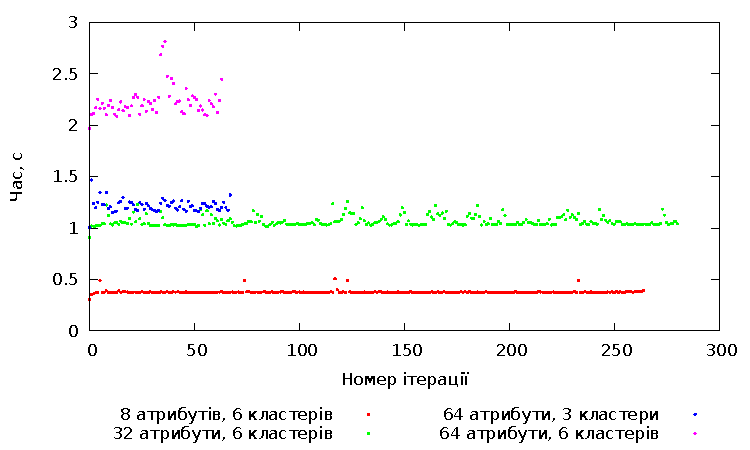
\includegraphics[scale=1.3]{kmeans_iteration_linear.pdf}
                    \caption{Графік залежності часу виконання ітерації k-means від її номера}\label{fig:kmeans_linear}
                \end{figure}
                
                На вхід алгоритму подавались три схожі синтетичні набори даних. Об’єкти в кожному з них розташовуються випадковим чином всередині n-вимірного куба з центром в початку координат та довжиною сторони, що дорівнює 2. Кількість об’єктів у кожному наборі --- 100000. Ці набори даних містили відповідно об’єкти з 8-вимірного, 32-вимірного та 64-вимірного просторів. Ці набори алгоритм повинен був розбити на 3 та 6 кластерів.
                
                \begin{figure}
                    \centering
                    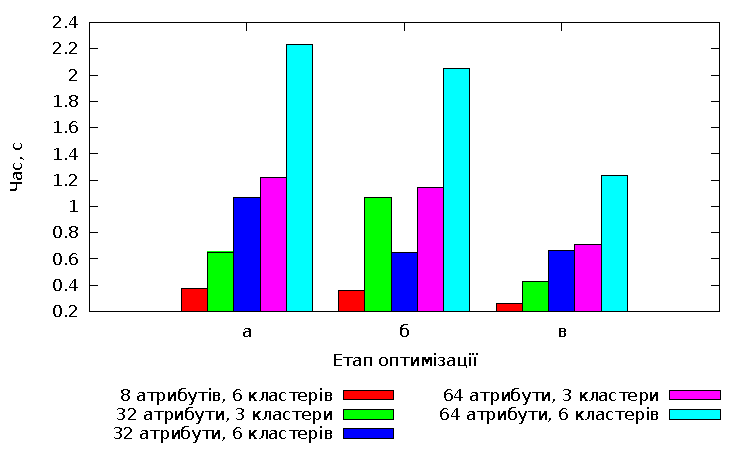
\includegraphics[scale=1.3]{kmeans_iteration_average.pdf}
                    \caption{Середній час виконання ітерацій k-means}\label{fig:kmeans_average}
                \end{figure}
                
                Рис.~\ref{fig:kmeans_average} показує середній час виконання ітерації k-means для різних вхідних даних. Рис.~\ref{fig:kmeans_average}, \emph{а} ілюструє роботу k-means у первинному вигляді. Рис.~\ref{fig:kmeans_average}, \emph{б} показує час роботи алгоритму після переходу на числа одинарної точності. Як бачимо, ця зміна суттєво вплинула лише на варіант запуску, що вимагав найбільше обчислень.
                
                Профілювання показало, що вибрана структура даних спричиняє великі втрати. За задумом, кожен екземпляр класу Object містив вектор екземплярів класу Attribute. Клас Attribute містив значення відповідного атрибуту та деяку додаткову інформацію (зокрема, дані про те, чи цей атрибут відомий із вхідного масиву). Це дозволяло легко розширити програму, додавши до неї функціонал передбачення даних, яких бракує у вибірці.
                
                За результатами профілювання від цеї структури довелось відмовитись. Замість вектора об’єктів використано динамічний масив чисел. Швидкість роботи k-means у такому випадку показано на рис.~\ref{fig:kmeans_average}, \emph{в}. Можна бачити, що така модифікація відчутно  зменшила час кожної ітерації.
                
            \section{DBSCAN}
                У DBSCAN кількість ітерацій рівна кількості об’єктів. На кожній ітерації вибирається один з об’єктів вибірки та обчислюються відстані від нього до усіх інших об’єктів вибірки. Таким чином, складність обчислень не змінюється між ітераціями. Проте, на відміну від k-means, залежно від результатів обчислень в ітерації можуть проводитись додаткові дії (такі як, наприклад, додавання сусідів об’єкта до списку об’єктів для подальшого аналізу). За рахунок додаткових операцій із пам’яттю ця особливість впливає на час роботи алгоритму. Відхилення від середнього значення часу виконання ітерації спостерігались в обидва боки (в менший бік, якщо в об’єкта немає достатньої кількості сусідів, і ніяк не впливає на список об’єктів для розгляду, і в більший, якщо об’єкт додає своїх сусідів до списку розгляду). Максимальний розмір відхилення --- 20\% від часу виконання ітерації.
                
                \begin{figure}
                    \centering
                    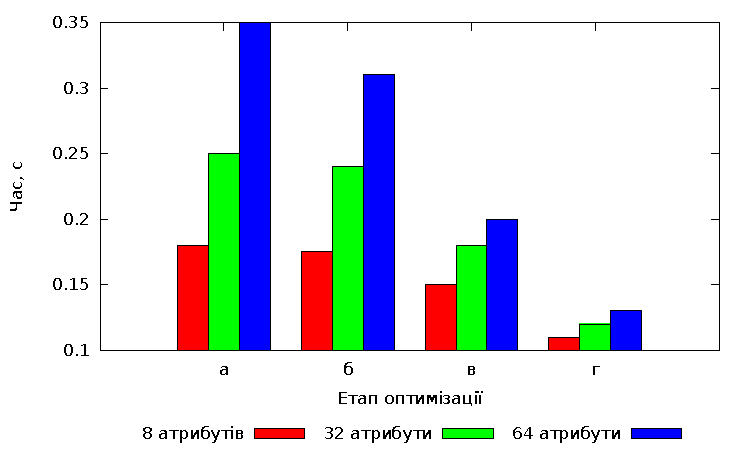
\includegraphics[scale=1.3]{dbscan_compare.pdf}
                    \caption{Середній час виконання ітерацій DBSCAN}\label{fig:dbscan_compare}
                \end{figure}
                
                На вхід алгоритму подавався той самий масив даних, що і для k-means. На рис.~\ref{fig:dbscan_compare} вказано середній час ітерації для кожного проведеного етапу оптимізації. На рис.~\ref{fig:dbscan_compare}, \emph{а} зображено час виконання одної ітерації для початкової версії алгоритму. Рис.~\ref{fig:dbscan_compare}, \emph{б} показує час виконання одної ітерації після переходу від чисел із подвійною точністю до чисел одинарної точності. Як і у випадку k-means, цей перехід мав суттєвий вплив лише на час обробки даних великої розмірності. Наступна група, рис.~\ref{fig:dbscan_compare}, \emph{в}, показує час виконання одної ітерації алгоритму після відмови від складної структури доступу до атрибутів об’єктів. Знову, аналогічно до k-means, цей перехід суттєво прискорив роботу алгоритму. Важливо звернути увагу на рис.~\ref{fig:dbscan_compare}, \emph{г}. Це --- результат оптимізації, що полягає у покращенні роботи з пам’яттю. Ця зміна призвела до зникнення залежності між кількістю близьких сусідів в об’єкта, що розглядається на певній ітерації, та часом виконання цеї ітерації. Такого покращення вдалось досягнути, відмовившись від деяких фактично зайвих операцій з пам’яттю.
                
            \subsection{UPGMA}
                UPGMA на кожній ітерації потребує матриці відстаней між усіма об’єктами вибірки. 

\bibliographystyle{gost780s}
\bibliography{chapters/bibliography/sources}


\end{document}
